\section{DSL + Types + Metadata == Business Modeling}\label{sec:03}

  There three principle compounds that are at the foundation of every business application based on the Trident Genesis platform: Domain Specific Languages, Type System and Metadata.
  Together they provide a uniform way of modeling the business domain.

\subsection{Domain Specific Languages}

  In recent years there was a spike in popularity of the Domain-Specific Languages (DSL) concept, which can be explainded by the programming issues outlined in section \ref{sec:01}, which affect not only the business oriented information systems, but also other domains dependent on various informations systems.

  The concept of DSL is not new.
  In fact, there are well established solutions for business software what exist for a long time and explictly utilise this concept.
  For example, SAP Business Suite offers a specialised language ABAP and Microsoft Dynamics Axapta provides X++.
  These are examples of so called \emph{external DSL}, which are separate or external to the programming language used natively for creation of the mentioned products.
  The main disadvantage with external DSLs is this: if there is a need to express a complex algorithm the expressive power of a DSL should be adequate to implement such algorithm, which in turn makes that DSL yet another general purpose programming language\footnote{External DSLs, which have the expressive power of general purpose languages have the disadvantage of being a lot less popular, making difficult to find experienced software developers to support existing systems.}.
  If the internal DSL is not expressive enough then developers would have to anyway resort to some general purpose programming language.

  An opposite to external DSL is the concept of \emph{interna DSL} -- a specialised language, which utilises the capabilities of a specific general purpose programming language (host language) of expressing language-like constructs that can be used together with the general purpose programming language.
  Internal DSLs share the development and execution infrastructure of the corresponding general purpose programming language taking a significant advantage of reusing debugging, profiling tools, code editors, existing programming libraries etc.

  \begin{wrapfigure}{l}{90mm}
    \centering    
    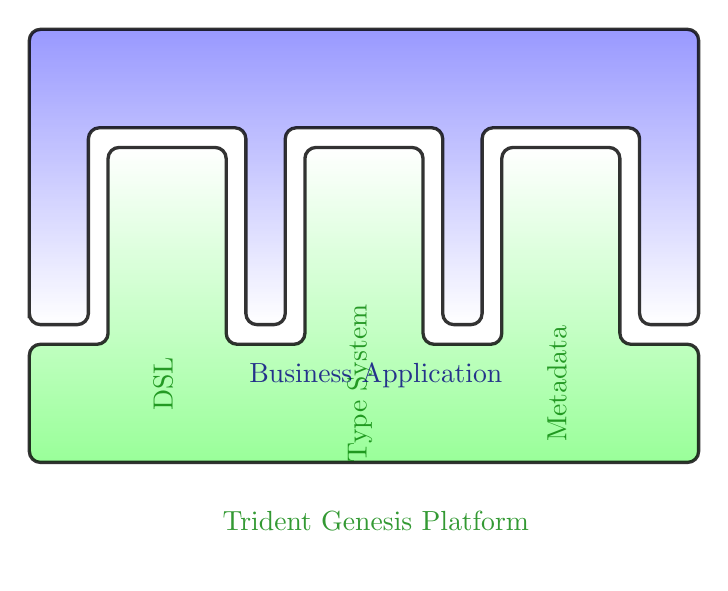
\begin{tikzpicture}[node distance=1cm, auto, opacity=0.8]
      \tikzset{
	  application/.style={rectangle,rounded corners,draw=black, top color=blue!50!white, bottom color=white,very thick, inner sep=1em, minimum size=3em, text centered, text=blue!50!black},
	  platform/.style={rectangle,rounded corners,draw=black, top color=white, bottom color=green!50!white,very thick, inner sep=1em, minimum size=3em, text centered, text=green!50!black},
	  mylabel/.style={text width=7em, text centered} 
      }  
      
      \def\platformpath{-- +(8.5cm,0cm) -- +(8.5cm,1.5cm) -- +(7.5cm,1.5cm) -- +(7.5cm,4.0cm) -- +(6.0cm,4.0cm) -- +(6.0cm,1.5cm) -- +(5.0cm,1.5cm) -- +(5.0cm,4.0cm) -- +(3.5cm,4.0cm) -- +(3.5cm,1.5cm) -- +(2.5cm,1.5cm) -- +(2.5cm,4.0cm) -- +(1.0cm,4.0cm) -- +(1.0cm,1.5cm) -- +(0.0cm,1.5cm) -- cycle}
      
      \draw (-1,-1.5) [platform] \platformpath
	    node [below, text width=3.5cm, text centered, yshift=1.0cm, xshift=1.15cm, rotate=90] {DSL}
	    node [below, text width=3.5cm, text centered, yshift=1.0cm, xshift=3.65cm, rotate=90] {Type System}
	    node [below, text width=3.5cm, text centered, yshift=1.0cm, xshift=6.15cm, rotate=90] {Metadata}
	    node [below, text centered,xshift=4.4cm, yshift=-0.2cm] {Trident Genesis Platform};

      \def\apppath{-- +(0cm,0cm) -- +(0.75cm,0cm) -- +(0.75cm,2.5cm) -- +(2.75cm,2.5cm) -- +(2.75cm,0cm) -- +(3.25cm,0cm) -- +(3.25cm,2.5cm) -- +(5.25cm,2.5cm) -- +(5.25cm,0cm)-- +(5.75cm,0cm)-- +(5.75cm,2.5cm) -- +(7.75cm,2.5cm) -- +(7.75cm,0cm) -- +(8.5cm,0cm) -- +(8.5cm,3.75cm) -- +(0cm,3.75cm) -- cycle}

      \draw (-1,0.25) [application] \apppath node [above, text centered,xshift=4.4cm, yshift=-1.2cm] {Business Application};
    \end{tikzpicture} 
  \end{wrapfigure}
  
  Different general purpose programming languages provide different degrees of support for developing sophisticated internal DSLs.
  For example, scripting languages generally provide better ways of implementing internal DSLs (e.g. Ruby).
  However, in our strong oppinion statically type langugages are of essential importantce for constructing complex business oriented information systems.
  
  From the very beginning the Trident Genesis Platform was envisaged as an application platform founded on concepts of the internal DSL and domain-driven development (inspired by Eric Evans's ``Domain-Driven Design: Tackling Complexity in the Heart of Software'').
  In order to ensure wider acceptance by the software development community\footnote{Popularisation of the paltform among developers and the existance of multiple business applications built on top of it forms a community, which provides an invaluable resource for new developers and helps identifying additional features that should be incorporated into the platform leading to further improvement of its abstraction mechanism.}, the platform taps into the power of modern IDEs and existing programming skills of softare developers using the Java programming language\footnote{Java is not the best host language for developing internal DSLs (e.g. Scala is a lot more adequate), but the maturity of the existing Java infrastructure and the development experience played a critical part in this decision.}.
  The internal DSLs are used for expressing the application's behaviour in a declarative way addressing key areas of any software solution such as web, database communication and the user interface desing.

\subsection{Type System and Metadata}
  The concept of \emph{metadata driven} software development is well accepted and repidly gaining its popularity among practitioners, affecting all modern software platforms and frameworks.
  The TG platform provides its unique type system and metadata support specifically targeted at the development of business applications.
  The core of any TG-based applications is formed out of types modeling the business entityes and the metadata, which complements the types.
  Together types and metadata define the object hierarchy used for building all main parts of the business application as well as for determining all aspect of its behaviour.
  Basically, the execution of such business applications effectively interprets the developed types and metadata, which provides all necessary application functionality.

  The business domain entities are modeled by reusing provided in the platform type system, which supports well-defined patterns for modeling real-life interoperability between domain entities.  
  Metadata privides a declarative way to associate various business rules with domain entities (e.g. validation rules), define application security, control transaction demracation, visual representation of domain entities and more.
  It also assists in fine-tuning of the business domain models with the support for configuration-based behaviour achieved by means of dependecy injection.
  
  By describing the application in terms of types and metadata, the developer informs the platform of a lot of useful information, which can be used by the platform in many different ways.
  Based on this information, the platform automatically constructs a large part of the application internals, which provides the support for a complete application lifecycle.
  For instance, provided metadata and types are sufficient for automatic construction of the application user interface that leverages the declared validation rules and dependencies between domain entities.
  Even more, the platform utilises this information for providing experienced end-users (i.e. without programming skills) of the business application with facilities to build comprehensive reports and analyses.

  So, be basic idea behind the type system and metadata driven approach to model the business domain is to depart from the old imperative paradigm towards the declarative way of defining the information system while remaining in the realm of the pure Java programming language\footnote{TG strives to confine the application development process to the use of Java only without the need for XML or any other external to Java language for modeling the business domain.}.
  
  

%   \begin{figure}[!htp]
%     \centering
%     
\includegraphics[width=10cm]{sections/01-intro/images/00-splash.jpg}
%     \caption{Example of an Embedded Image}\label{fig:01}
%   \end{figure}


%  // calculates the average yearly maintenance cost (for the last 3 years) per sectors of NORTH division. Only vehicles of MERCEDES make and models starting from 315 or 316 or VITO model are taken into account.
%         select(WorkOrder.class).
%         where(). //
%         prop("vehicle.model.make.key").eq().val("MERCEDES").and().
%         begin().prop("vehicle.model.key").starts_with().any_of_values("315", "316" ).or().prop("vehicle.model.key").eq().val("VITO").end().and().
%         year_of().prop("actualStart").in().values(2009, 2010, 2011).and().
%         prop("vehicle.station.zone.sector.division.key").eq().val("NORTH").
%         yield_and_group().prop("vehicle.station.zone.sector").as("sector").
%         yield().begin_expr().sum_of().prop("actualCost").div().val(3).end_expr().as("averageYearlyMaintenanceCostPerSector").model_as_aggregate();
 